%------- ------- ------- Document Headers
\documentclass[10pt]{article} % latexmk, pdflatex
\usepackage[includefoot, paperheight=297mm, paperwidth=210mm, textwidth=170mm, textheight=257mm]{geometry} % texlive-geometry
\usepackage{lastpage} % texlive-lastpage
\usepackage{fancyhdr} % texlive-fancyhdr
\usepackage{graphicx} % 
\usepackage{indentfirst} % 
\usepackage{longtable} % 
\usepackage{array} % 
\usepackage{multicol} % 
\usepackage{multirow} % texlive-multirow
\usepackage{enumitem} % texlive-enumitem
\usepackage{mathtools} % texlive-mathtools
\usepackage{amsfonts} % texlive-amsfonts
\usepackage{amssymb} % 
\usepackage{hyperref} % texlive-hyperref
\usepackage{titlesec} % texlive-titlesec
\usepackage{tikz} % 
\usepackage{tkz-euclide} % texlive-tkz-euclide
%------- ------- ------- Initialization
\setlength{\parindent}{32pt}
\renewcommand{\baselinestretch}{0.7}
\renewcommand{\contentsname}{Sumário}
%------- ------- fancyhdr
\pagestyle{fancy}
\fancyhf{}
\renewcommand{\headrulewidth}{0pt}
\fancyfoot[R]{\thepage \hspace{1pt} / \pageref*{LastPage}}
%------- ------- array
\renewcommand{\arraystretch}{2}
%------- ------- multicol
\setlength{\columnsep}{32pt}
%------- ------- enumerate
\setlist{noitemsep, left=64pt}
%------- ------- hyperref
\hypersetup{colorlinks=true, linkcolor=blue, pdfpagemode=FullScreen, pdftitle={Annotationes Meae}, pdfauthor={Gustavo Aragão}}
%------- ------- titlesec
\titleformat{\section}[block]{\normalfont\Large\bfseries}{\thesection}{16pt}{}
\titleformat{\subsection}[block]{\normalfont\large\bfseries}{\hspace{16pt}\thesubsection}{16pt}{}
\titleformat{\subsubsection}[block]{\normalfont\bfseries}{\hspace{32pt}\thesubsubsection}{16pt}{}
%------- ------- tikz
\usetikzlibrary{matrix}
\pgfdeclarelayer{bg}
\pgfdeclarelayer{fg}
\pgfsetlayers{bg,main,fg}
%------- ------- Commands
\newcommand{\eg}{\textit{e.g.:}}
%------- ------- ------- Beginning of Document
\begin{document}
    %------- ------- Title
    \title{
        \begin{tikzpicture}[scale=0.3, line join=bevel]
            % \a and \b are two macros defining characteristic
            % dimensions of the Penrose triangle.		
            \pgfmathsetmacro{\a}{2.5}
            \pgfmathsetmacro{\b}{0.9}
    
            \tikzset{
              apply style/.code     = {\tikzset{##1}},
              triangle_edges/.style = {thick,draw=black}
            }
    
            \foreach \theta/\facestyle in {
                0/{triangle_edges, fill = gray!50},
                120/{triangle_edges, fill = gray!25},
                240/{triangle_edges, fill = gray!90}
            }{
                \begin{scope}[rotate=\theta]
                    \draw[apply style/.expand once=\facestyle]
                    ({-sqrt(3)/2*\a},{-0.5*\a})                     --
                    ++(-\b,0)                                       --
                    ({0.5*\b},{\a+3*sqrt(3)/2*\b})                -- % higher point	
                    ({sqrt(3)/2*\a+2.5*\b},{-.5*\a-sqrt(3)/2*\b}) -- % rightmost point
                    ++({-.5*\b},-{sqrt(3)/2*\b})                    -- % lower point
                    ({0.5*\b},{\a+sqrt(3)/2*\b})                  --
                    cycle;
                \end{scope}
            }	
        \end{tikzpicture} \\
        \vspace{8pt} Annotationes Meae \\ Mathematicae
    }
    \author{\textit{Gustavo Aragão}}
    \date{}
    \maketitle
    \thispagestyle{fancy}
    %------- ------- Table of Contents
    \tableofcontents
    \newpage
    %------- ------- 1
    \section{Lógica e Notação}
    %------- 1.1
\subsection{Conectivos}
    \begin{center}
        \begin{longtable}{| m{3cm} | m{12cm} |}
                \hline $ \neg $ & Negação\\
                \hline $ \vee $ & Disjunção\\
                \hline $ \wedge $ & Conjunção\\
                \hline $ \rightarrow $ & Implicação; Condicional\\
                \hline $ \leftrightarrow $ & Bi-implicação; Equivalência\\
                \hline
            \end{longtable}
    \end{center}
%------- 1.2
\subsection{Quantificadores}
    \begin{center}
        \begin{longtable}{| m{3cm} | m{12cm} |}
            \hline $ \forall $ & Todo; Qualquer\\
            \hline $ \exists $ & Existe; Pelo menos um; Algum\\
            \hline $ \exists ! $ & Existe exatamente um\\
            \hline
        \end{longtable}
    \end{center}
%------- 1.3
\subsection{Pontuações}
    \begin{center}
        \begin{longtable}{| m{3cm} | m{12cm} |}
            \hline $ \pm $ & Mais ou menos\\
            \hline $ = $ & Igual\\
            \hline $ \neq $ & Diferente\\
            \hline $ \equiv $ & Equivalente; Congruente\\
            \hline $ \sim $ & Aproximadamente\\
            \hline $ \approx $ & Aproximadamente igual\\
            \hline $ > $ & Maior que\\
            \hline $ \geq $ & Igual ou maior que\\
            \hline $ < $ & Menor que\\
            \hline $ \leq $ & Igual ou menor que\\
            \hline $ \star $ & Igual, maior ou menor que\\
            \hline $ \prec $ & Sequencialmente precede\\
            \hline $ \succ $ & Sequencialmente sucede\\
            \hline $ \propto $ & Proporcional\\
            \hline $ | $ & Tal que\\
            \hline $ ( ), [ ], \{ \} $ & Delimitadores\\
            \hline $ (\cdots)_p $ & Enupla de $p$ elementos\\
            \hline $ \{\cdots\} $ & Conjunto\\
            \hline $ \varnothing, \{\} $ & Conjunto vazio\\
            \hline $ \# $ & Número de elementos contidos\\
            \hline $ \nexists $ & Não existe\\
            \hline $ \ni, \supset $ & Contém\\
            \hline $ \not\ni, \not\supset $ & Não contém\\
            \hline $ \in, \subset $ & Está contido\\
            \hline $ \notin, \not\subset  $ & Não está contido\\
            \hline $ \supset $ & É subconjunto\\
            \hline $ \subset $ & É superconjunto\\
            \hline $ \cup $ & União\\
            \hline $ \cap $ & Interseção\\
            \hline $ \mathcal{P} $ & Propriedade; Lei de aplicação\\
            \hline $ \mathcal{D} $ & Domínio\\
            \hline $ \mathcal{CD} $ & Contradomínio\\
            \hline $ \mathcal{IM} $ & Imagem\\
            \hline $ \mathcal{C}^{B}_{A} $ & Complementar de $B$ em $A$\\
            \hline $ A^* $ & Conjunto dos elementos não nulos de $A$\\
            \hline $ A^n $ & Conjunto dos $n$ primeiros elementos de $A$\\
            \hline $ A_+ $ & Conjunto dos elementos positivos de $A$\\
            \hline $ A_- $ & Conjunto dos elementos negatios de $A$\\
            \hline $ \mathbb{N} $ & Conjunto dos números naturais\\
            \hline $ \mathbb{Z} $ & Conjunto dos números inteiros\\
            \hline $ \mathbb{Q} $ & Conjunto dos números racionais\\
            \hline $ \mathbb{I} $ & Conjunto dos números irracionais\\
            \hline $ \mathbb{R} $ & Conjunto dos números reais\\
            \hline $ \mathfrak{I} $ & Conjunto dos números imaginários\\
            \hline $ \mathbb{C} $ & Conjunto dos números complexos\\
            \hline $ \mathbb{U} $ & Conjunto universo\\
            \hline $ \mapsto $ & Função aplicada\\
            \hline $ \mathrm{P}(n) $ & Polinômio de Grau $n$\\
            \hline $ \therefore $ & Portanto\\
            \hline $ \because $ & Em razão de\\
            \hline $ \infty $ & Infinito\\
            \hline $ \Delta $ & Variação\\
            \hline $ \lim\limits_{a \to b} f(x) $ & Limite\\
            \hline $ f', \frac{dy}{dx} $ & Derivada\\
            \hline $ \frac{\partial y}{\partial x}  $ & Derivada parcial\\
            \hline $ \int_a^b $ & Integral\\
            \hline $ \oint_a^b $ & Integral de linha\\
            \hline $ \nabla $ & Gradiente\\
            \hline $ \displaystyle\sum_{i=a}^{b} f(i) $ & Somatório\\
            \hline $ \displaystyle\prod_{i=a}^{b} f(i) $ & Produtório\\
            \hline $ \mathring{APB} $ & Ponto $P$ contido entre $A$ e $B$\\
            \hline $ \overline{AB} $ & Segmento de reta\\
            \hline $ \overrightarrow{AB} $ & Semirreta\\
            \hline $ \hat{\alpha}, \hat{AOB} $ & Ângulo\\
            \hline $ \parallel $ & Paralelo\\
            \hline $ \nparallel $ & Concorrente\\
            \hline $ \bot $ & Perpendicular\\
            \hline $ \triangle ABC $ & Triângulo ABC\\
            \hline $ \Diamond ABCDE $ & Polígono ABCDE\\
            \hline
        \end{longtable}
    \end{center}
%------- 1.4
\subsection{Alfabeto Grego}
    \begin{center}
        \begin{longtable}{| m{3cm} | m{3cm} | m{8.57cm} |}
            \hline $ \alpha $ & $ A $ & Alfa\\
            \hline $ \beta $ & $ B $ & Beta\\
            \hline $ \gamma $ & $ \Gamma $ & Gama\\
            \hline $ \delta $ & $ \Delta $ & Delta\\
            \hline $ \epsilon $ & $ E $ & Epsilon\\
            \hline $ \zeta $ & $ Z $ & Zeta\\
            \hline $ \eta $ & $ H $ & Eta\\
            \hline $ \theta $ & $ \Theta $ & Theta\\
            \hline $ \iota $ & $ I $ & Iota\\
            \hline $ \kappa $ & $ K $ & Kappa\\
            \hline $ \lambda $ & $ \Lambda $ & Lambda\\
            \hline $ \mu $ & $ M $ & Mu\\
            \hline $ \nu $ & $ N $ & Nu\\
            \hline $ \xi $ & $ \Xi $ & Xi\\
            \hline $ o $ & $ O $ & Omicron\\
            \hline $ \pi $ & $ \Pi $ & Pi\\
            \hline $ \rho $ & $ P $ & Rho\\
            \hline $ \sigma $ & $ \Sigma $ & Sigma\\
            \hline $ \tau $ & $ T $ & Tau\\
            \hline $ \upsilon $ & $ \Upsilon $ & Upsilon\\
            \hline $ \phi $ & $ \Phi $ & Phi\\
            \hline $ \chi $ & $ X $ & Chi\\
            \hline $ \psi $ & $ \Psi $ & Psi\\
            \hline $ \omega $ & $ \Omega $ & Omega\\
            \hline
        \end{longtable}
    \end{center}
    %------- ------- 2
    \section{Teoria dos Conjuntos}
    %------- 2.1
\subsection{Conceitos Básicos}
    %--- 2.1.1
    \subsubsection{Definição}
        Conjunto é um agrupamento de elementos, aleatórios ou selecionados criteriosamente por um sistema. Pode ser enumerado ou ter seus critérios descritos em propriedades. \eg
        \[ A = \{ 0,1,2,3,5,8,13 \}; A = \{ x \in \mathbb{U} | \mathcal{P} \} \]
    %--- 2.1.2
    \subsubsection{Tipos}
        \begin{description}
            \item[Conjunto Unitário] é aquele que possui um único elemento. \eg \hfill $ A = \{7\} $
            \item[Conjunto Vazio] é aquele que não possui elemento algum. \eg \hfill $ A = \{  \}; A = \varnothing $
            \item[Conjunto Universo] é aquele que contém todos os elementos utilizados no assunto
tratado
        \end{description}
    %--- 2.1.3
    \subsubsection{Intervalos}
        Definido como uma descrição de conjunto que compreende todos os números em determinado espaço da reta numérica (considerado o conjunto universo), podendo ser abertos ou fechados. \eg
        \[ (a<b) \]
        \[ ]a,b[ = \{ x \in \mathbb{U} | a < x < b \} \]
        \[ [a,b] = \{ x \in \mathbb{U} | a \leq x \leq b \} \]
        
        Intervalos possuem uma representação gráfica na reta numérica. \eg
        \begin{center}
            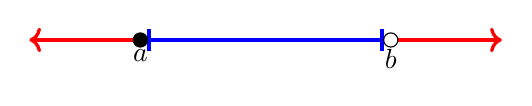
\begin{tikzpicture}
                \draw[red, very thick, <->] (-3,0) -- (3,0);
                \draw[blue, very thick, |-|] (-1.5,0) -- (1.5,0);
                \filldraw[color=black, fill=black] (-1.59,0) circle (0.09) node[below]{$a$};
                \filldraw[color=black, fill=white, thin] (1.59,0) circle (0.09) node[below]{$b$};
            \end{tikzpicture}
            \[ [a,b[ = \{ x \in \mathbb{R} | a \leq x < b \} \]
        \end{center}
    %--- 2.1.4
    \subsubsection{Pares Ordenados}
        Chama-se par ordenado o conjunto de 2 elementos onde sua ordem importa:
        \[ (a,b) = \{ \{ a \}, \{ a, b \} \} \]
        \[ (a,b) = (c,d) \rightarrow a = c \wedge b = d \]
        
        Muito utilizado para a representação de pontos em um plano cartesiano, indicando sua abscissa e sua ordenada, respectivamente:
        \[ P \in \alpha = (x_p, y_p) \]
    %--- 2.1.5
    \subsubsection{Produto Cartesiano}
        Considerando os conjuntos não vazios A e B, o produto cartesiano de A por B é o conjunto cujos elementos são todos os pares ordenados onde o primeiro elemento pertence a A e o segundo a B:
        \[ (A, B \neq \varnothing) \]
        \[ A \times B = \{ (x,y) | x \in A \wedge y \in B \} \]
    %--- 2.1.6
    \subsubsection{Relação Binária}
        A relação binária é um subconjunto criterioso dos elementos de um produto cartesiano definido por uma lei de aplicação:
        \[ R_{A \times B} = \{ (x,y) \in A \times B | \mathcal{P} \} \]
    %--- 2.1.7
    \subsubsection{Domínio}
        Na relação binária de A em B, o domínio é o subconjunto de todos os elementos de A que tenham uma aplicação em B:
        \[ x \in \mathcal{D}(R_{A \times B}) \leftrightarrow \exists y \in B | (x,y) \in R_{A \times B} \]
    %--- 2.1.8
    \subsubsection{Contradomínio}
        Na relação binária de A em B, o contradomínio é simplesmente B, sendo o conjunto de chegada da lei de aplicação:
        \[ \mathcal{CD}(R_{A \times B}) = B \]
    %--- 2.1.9
    \subsubsection{Imagem}
        Na relação binária de A em B, a imagem é o subconjunto do contradomínio formado por todos os elementos que sejam associados ao domínio pela lei de aplicação:
        \[ y \in \mathcal{IM}(R_{A \times B}) \leftrightarrow \exists x \in A | (x,y) \in R_{A \times B} \]
    %--- 2.1.10
    \subsubsection{Relação Inversa}
        Dada a relação binária de A em B, a sua relação inversa é a aplicação de sua lei no produto cartesiano de B por A:
        \[ R^{-1}_{A \times B} = \{ (y,x) \in B \times A | (x,y) \in R_{A \times B} \} \]
%------- 2.2
\subsection{Relações}
    %--- 2.2.1
    \subsubsection{Subconjuntos}
        Um conjunto A é subconjunto de outro conjunto B se todo elemento que pertencente a A também pertence a B:
        \[ A \subset B \leftrightarrow \forall x \in A, B \ni x \]
    %--- 2.2.2
    \subsubsection{Igualdade}
        Dois conjuntos A e B são classificados como iguais quando todo elemento de A pertence a B, e todo elemento de B pertence a A:
        \[ A = B \leftrightarrow (\forall x \in A, B \ni x) \wedge (\forall y \in B, A \ni y) \]
    %--- 2.2.3
    \subsubsection{Reunião}
        Chama-se reunião de A e B o conjunto formado pelos elementos que pertencem a A ou a B:
        \[ A \cup B = \{ x | x \in A \vee x \in B \} \]
    %--- 2.2.4
    \subsubsection{Interseção}
        Chama-se interseção de A e B o conjunto formado pelos elementos que pertencem a A e a B:
        \[ A \cap B = \{ x | x \in A \wedge x \in B \} \]

        Conjuntos que não possuem elementos em comum são chamados conjuntos distintos.
    %--- 2.2.5
    \subsubsection{Diferença}
        Chama-se diferença entre A e B o conjunto formado pelos elementos de A que não pertencem a B:
        \[ A - B = \{ x | x \in A \wedge x \notin B \} \]
    %--- 2.2.6
    \subsubsection{Complementar}
        Considerando um conjunto A e seu subconjunto B, chama-se o complementar de B em relação a A o conjunto dos elementos de A que não pertencem a B:
        \[ (B \subset A) \]
        \[ \mathcal{C}^{B}_{A} = A - B \]
    %--- 2.2.7
    \subsubsection{Propriedades}
        Considerando A, B e C como conjuntos quaisquer:
        \begin{multicols}{3}
            \noindent\[ \varnothing \subset A \]
            \[ A \subset A \]
            \[ A \cup A = A \]
            \[ A \cap A = A \]
            \[ A \cup \varnothing = A \]
            \[ A \cap \varnothing = A \]
            \[ A \cup B = B \cup A \]
            \[ A \cap B = B \cap A \]
            \[ (A \subset B) \wedge (A \supset B) \leftrightarrow A = B \]
            \[ (A \subset B) \wedge (B \subset C) \rightarrow A \subset C \]
            \[ (A \cup B) \cup C = A \cup (B \cup C) \]
            \[ (A \cap B) \cap C = A \cap (B \cap C) \]
        \end{multicols}
        Considerando A e seus subconjuntos B e C:
        \[ (A \supset B,C) \]
        \[ \mathcal{C}^{B}_{A} \cup B = A; \mathcal{C}^{B}_{A} \cap B = \varnothing \]
%------- 2.3
\subsection{Conjuntos Numéricos}
    %--- 2.3.1
    \subsubsection{Naturais}
        O conjunto dos números naturais define-se em:
        \[ \mathbb{N} = \{ 1,2,3,... \} \]
    %--- 2.3.2
    \subsubsection{Inteiros}
        O conjunto dos números inteiros estende o conjunto dos naturais com números negativos:
        \[ \mathbb{Z} = \{ ...,-1,0,1,2,... \} \]
    %--- 2.3.3
    \subsubsection{Racionais}
        O conjunto dos números racionais estende o conjunto dos inteiros com a representação de componentes fracionários:
        \[ \mathbb{Q} = \left\{\frac{a}{b} | a \in \mathbb{Z} \wedge b \in \mathbb{Z}^* \right\} \]
    %--- 2.3.4
    \subsubsection{Irracionais}
        O conjunto dos números irracionais compreende os números da reta numérica que não podem ser representados por frações, sendo dízimas não periódicas sem uma razão numérica:
        \[ \mathbb{I} = \left\{ x | \frac{p}{q} \neq x \ \forall p,q \in \mathbb{Z} \right\} \]
    %--- 2.3.5
    \subsubsection{Reais}
        O conjunto dos números reais engloba todos os números existentes na reta numérica, sendo a união do conjunto dos racionais com o conjunto dos irracionais:
        \[ \mathbb{R} = \mathbb{Q} \cup \mathbb{I} \]
    %--- 2.3.6
    \subsubsection{Imaginários}
        O conjunto dos números imaginários traz o conceito de perpendicularidade para a reta numérica:
        \[ \mathfrak{I} = \left\{ \sqrt[n]{m} | \frac{n}{2} \in \mathbb{Z} \wedge m \in \mathbb{Z}^*_- \right\} \]
    %--- 2.3.7
    \subsubsection{Complexos}
        O conjunto dos números complexos é a conjunção dos números reais e imaginários, transformando a reta numérica em um plano:
        \[ \mathbb{C} = \{ (x,y) | x \in \mathbb{R} \wedge y \in \mathfrak{I} \} \]
    %------- ------- 3
    \section{Aritmética}
    %%------- 3.1
\subsection{Princípoos da Dinâmica}
    \[ \Upsilon \pi o \mu o \nu \eta \]
%------- 3.2
\subsection{Movimento Linear Uniforme}
    \[ \Upsilon \pi o \mu o \nu \eta \]
%------- 3.3
\subsection{Movimento Angular Uniforme}
    \[ \Upsilon \pi o \mu o \nu \eta \]
%------- 3.4
\subsection{Energia Mecânica}
    \[ \Upsilon \pi o \mu o \nu \eta \]
%------- 3.5
\subsection{Colisões}
    \[ \Upsilon \pi o \mu o \nu \eta \]
    %------- ------- 4
    \section{Álgebra Elementar}
    %%------- 4.1
\subsection{Hidrostática}
    \[ \Upsilon \pi o \mu o \nu \eta \]
%------- 4.2
\subsection{Noções de Hidrodinâmica}
    \[ \Upsilon \pi o \mu o \nu \eta \]
%------- 4.3
\subsection{Gases}
    \[ \Upsilon \pi o \mu o \nu \eta \]
    %------- ------- 5
    \section{Álgebra Linear}
    %%------- 5.1
\subsection{Matrizes}
    %--- 5.1.1
    \subsubsection{Definição}
        Matriz é toda tabela formada por números reais, caracterizada pelo número de linhas e colunas, respectivamente, contadas de cima para baixo e da esquerda para direita:
        \[ (x, y, i, j \in \mathbb{N}) \]
        \[ M_{y \times x} = \begin{bmatrix} a_{1 \; 1} & & a_{1 \; x} \\ & \cdots & \\ a_{y \; 1} &  & a_{y \; x} \end{bmatrix} \ | \ a_{i \; j} \in \mathbb{R} \ \forall i \in \mathbb{N}^y \wedge  \forall j \in \mathbb{N}^x \]
    %--- 5.1.2
    \subsubsection{Classificações}
        \begin{description}
            \item[Matriz Nula:] é toda matriz onde todos os seus elementos são iguais a zero:
            \[ M_{y \times x} = \{a_{i \; j} = 0 \ | \ \forall i \in \mathbb{N}^y \wedge  \forall j \in \mathbb{N}^x \} \]
            \item[Matriz Linha:] é toda matriz que composta por uma única linha. \eg
            \[ M_{1 \times x} = \begin{bmatrix} a_{1 \; 1} & \cdots & a_{1 \; x} \end{bmatrix} \]
            \item[Matriz Coluna:] é toda matriz que composta por uma única coluna. \eg
            \[ M_{y \times 1} = \begin{bmatrix} a_{1 \; 1} \\ \vdots \\ a_{y \; 1} \end{bmatrix} \]
            \item[Matriz Quadrada:] é toda matriz com o mesmo número de linhas e colunas, onde este número é apontado como o seu grau. \eg
            \[ M_{n \times n} = \begin{bmatrix} a_{1 \; 1} & & a_{1 \; n} \\ & \cdots & \\ a_{n \; 1} &  & a_{n \; n} \end{bmatrix} \]
            Na matriz quadrada denota-se a importância de suas duas diagonais, a principal e secundária, respectivamente:
            \[ a_{i \; j} \in M_{n \times n} \ | \ i = j \hphantom{---} a_{i \; j} \in M_{n \times n} \ | \ i + j = n + 1 \]
            \item[Matriz Diagonal:] é toda matriz quadrada onde os elementos não pertencentes a diagonal principal são nulos. \eg
            \[ \begin{bmatrix} a_{1 \; 1} & 0 & 0 \\ 0 & a_{2 \; 2} & 0 \\ 0 & 0 & a_{3 \; 3} \end{bmatrix} \]
            \item[Matriz Identidade:] é toda matriz quadrada onde os elementos da diagonal principal são iguais a 1, enquanto todos os outros elementos são nulos. \eg
            \[ I_3 = \begin{bmatrix} 1 & 0 & 0 \\ 0 & 1 & 0 \\ 0 & 0 & 1 \end{bmatrix} \]
            \item[Matriz Triangular:] toda matriz quadrada onde os elementos acima ou abaixo da diagonal principal são nulos:
            \[ a_{i \; j} = 0 \ \forall i < j \vee j > i \]
        \end{description}
    %--- 5.1.3
    \subsubsection{Adição}
        A soma de duas matrizes (necessariamente de mesma dimensão) é feita pela soma de seus respectivos termos:
        \[ A_{y \times x} + B_{y \times x} = C_{y \times x} \ | \ c_{i \; j} = b_{i \; j} + a_{i \; j} \]
    %--- 5.1.4
    \subsubsection{Multiplicação}
        \begin{description}
            \item[Por um Coeficiente:] a multiplicação de uma matriz por um número é feita multiplicando cada um de seus elementos pelo coeficiente: 
            \[ A_{y \times x} \cdot k = B_{y \times x} \ | \ b_{i \; j} = k \cdot a_{i \; j} \]
            \item[Por Outra Matrix:] a multiplicação de duas matrizes (necessariamente tendo o número de colunas da primeira igual ao número de linhas da segunda) resulta numa matriz contendo a somatório do produto dos elementos ordenados em linha por coluna:
            \[ A_{m \times n} \cdot B_{n \times p} = C_{m \times p} \ | \ c_{i \; j} = \displaystyle\sum_{k=1}^{n} {a_{i \; k} \cdot b_{k \; j}} \]
            Nota-se que: $ M_{y \times x} \cdot I_y = I_y \cdot M_{y \times x} = M_{y \times x} $
        \end{description}
    %--- 5.1.5
    \subsubsection{Transposição}
        A transposição de uma matriz é seu espelhamento, invertendo a indexação de linhas e colunas de seus elementos:
        \[ M_{y \times x} = a_{i \; j} \xrightarrow{\text{transposição}} M_{x \times y}^t = a_{j \times i} \]
        Frente ao processo de transposição matricial, surgem duas classificações:
        \begin{description}
            \item[Matriz Simétrica:] é toda matriz quadrada equivalente a sua transposição.
            \item[Matriz Antissimétrica:] é toda matriz quadrada cuja qual, quando transposta, resulta na sua matriz oposta.
        \end{description}
        %--- 5.1.6
        \subsubsection{Inversão}
        Uma matriz quadrada é dita inversível quando existe uma inversa que multiplicada por ela resulta numa matriz identidade de mesma ordem:
        \[ M_{n \times n} \cdot M_{n \times n}^{-1} = M_{n \times n}^{-1} \cdot M_{n \times n} = I_n \]
%------- 5.2
\subsection{Determinantes}
    %--- 5.2.1
    \subsubsection{Definição}
        O determinante é uma função matricial que associa matrizes quadradas a um escalar que a define e mede sua transformação no espaço vetorial, possuindo inúmeras aplicações em campos diversos da matemática e física. Para matrizes de primeira e segunda ordem, o determinante é encontrado da seguinte forma:
        \[ \det{M_{1 \times 1}} = \begin{vmatrix} a_{1 \; 1} \end{vmatrix} = a_{1 \; 1} \]
        \begin{center}
            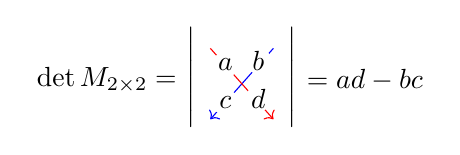
\begin{tikzpicture}
                \begin{pgfonlayer}{fg}
                    \matrix (M) [matrix of math nodes, left delimiter  = |, right delimiter = |] at (0,0) { a & b  \\ c & d \\ } node [left=20pt] {$ \det{M_{2 \times 2}} = $} node[right=20pt] {$ = ad - bc $};
                \end{pgfonlayer}
                \begin{pgfonlayer}{main}
                    \node[circle, fill=white] at (M-1-1) {};
                    \node[circle, fill=white] at (M-1-2) {};
                    \node[circle, fill=white] at (M-2-1) {};
                    \node[circle, fill=white] at (M-2-2) {};
                \end{pgfonlayer}
                \begin{pgfonlayer}{bg}
                    \draw[blue, ->] (0.4,0.4) -- (-0.4,-0.5);
                    \draw[red, ->] (-0.4,0.4) -- (0.4,-0.5);
                \end{pgfonlayer}
            \end{tikzpicture}
        \end{center}
    %--- 5.2.2
    \subsubsection{Regra de Sarrus}
        Para matrizes de terceira ordem, usamos a seguinte regra:
        \begin{center}
            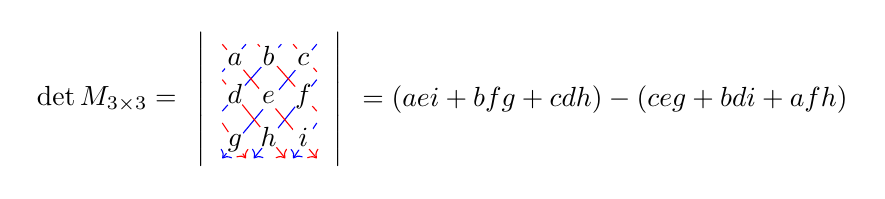
\begin{tikzpicture}
                \begin{pgfonlayer}{fg}
                    \matrix (M) [matrix of math nodes, left delimiter  = |, right delimiter = |] at (0,0) { a & b & c \\ d & e & f \\ g & h & i \\ } node [left=30pt] {$ \det{M_{3 \times 3}} =  $} node[right=30pt] {$ = (aei + bfg + cdh) - (ceg + bdi + afh) $};
                \end{pgfonlayer}
                \begin{pgfonlayer}{main}
                    \node[circle, fill=white] at (M-1-1) {};
                    \node[circle, fill=white] at (M-1-2) {};
                    \node[circle, fill=white] at (M-1-3) {};

                    \node[circle, fill=white] at (M-2-1) {};
                    \node[circle, fill=white] at (M-2-2) {};
                    \node[circle, fill=white] at (M-2-3) {};

                    \node[circle, fill=white] at (M-3-1) {};
                    \node[circle, fill=white] at (M-3-2) {};
                    \node[circle, fill=white] at (M-3-3) {};
                \end{pgfonlayer}
                \begin{pgfonlayer}{bg}
                    \draw[blue, ->] (0.6,0.7) -- (-0.6,-0.75);
                    \draw[blue, -] (0.15,0.7) -- (-0.6,-0.15);
                    \draw[blue, -] (-0.3,0.7) -- (-0.6,0.35);
                    \draw[blue, ->] (0.6,0.25) -- (-0.2,-0.75);
                    \draw[blue, ->] (0.6,-0.3) -- (0.3,-0.75);

                    \draw[red, ->] (-0.6,0.7) -- (0.6,-0.75);
                    \draw[red, -] (-0.15,0.7) -- (0.6,-0.15);
                    \draw[red, -] (0.3,0.7) -- (0.6,0.35);
                    \draw[red, ->] (-0.6,0.25) -- (0.2,-0.75);
                    \draw[red, ->] (-0.6,-0.3) -- (-0.3,-0.75);
                \end{pgfonlayer}
            \end{tikzpicture}
        \end{center}
    %--- 5.2.3
    \subsubsection{Menor Complementar}
        Para uma matriz de ordem maior que 2, o complementar algébrico de um elemento é o determinante que se obtém ao suprimir a linha e coluna desse elemento. \eg
        \[ M_{3 \times 3} = \begin{vmatrix} a & b & c \\ d & e & f \\ g & h & i \\ \end{vmatrix} : D_{1 \; 1} =  \begin{vmatrix} e & f\\ h & i\end{vmatrix}; D_{2 \; 2} =  \begin{vmatrix} a & c\\ g & i \end{vmatrix}; D_{3 \; 3} =  \begin{vmatrix} a & b \\ d & e \end{vmatrix} \]
        %--- 5.2.4
        \subsubsection{Complemento Algébrico}
        Para uma matriz de ordem maior que 2, o complemento algébrico (cofator) de um elemento é dado por:
        \[ A_{i \; j} = (-1)^{i + j} \cdot D_{i \; j} \]
    %--- 5.2.5
    \subsubsection{Determinante por Recorrência}
        A definição da determinante por recorrência (caso geral) é dada pela soma dos produtos dos elementos da primeira coluna por seus complementos algébricos:
        \[ \det{M_{n \times n}} = \displaystyle\sum_{i=i}^{n} {a_{i \; 1} \cdot A_{i \; 1} } \]
    %--- 5.2.6
    \subsubsection{Teorema de Laplace}
        O teorema de Laplace diz que o determinante de uma matriz de ordem maior que 2 é a soma dos produtos dos elementos de uma fila qualquer por seus respectivos cofatores, assim a definição do determinante por recorrência não precisa ser aplicado necessariamente à primeira coluna, mas a qualquer linha ou coluna de uma matriz.
    %--- 5.2.7
    \subsubsection{Combinação Linear}
        Define-se pelo conjunto das somas dos produtos dos elementos de determinadas filas por determinadas constantes, ordenadamente:
        \[ M_{n \times n} = [a_{i \; j}] \hphantom{---} s=\{filas \: paralelas \} \hphantom{---} p = \# s \hphantom{---} c = \{ c_1,...,c_p \}\]
        \[ \alpha = \{ \alpha_1, ..., \alpha_n \} \ | \ \alpha_{\sigma} =  \begin{dcases}  \displaystyle\sum_{k=1}^{p} {a_{s_k \; \sigma} \cdot c_k} \because s = \{linhas\} \\ \displaystyle\sum_{k=1}^{p} {a_{\sigma \; s_k} \cdot c_k} \because s = \{colunas\} \end{dcases} \]

        \eg
        \[ M_{3 \times 3} = [a_{i \; j}] \]
        \[ s_{x} = \{ 2,3 \}, c=\{q,r\} \rightarrow \alpha = \begin{dcases} \alpha_1 = a_{2 \; 1} \cdot q + a_{3 \; 1} \cdot r \\ \alpha_2 = a_{2 \; 2} \cdot q + a_{3 \; 2} \cdot r \\ \alpha_3 = a_{2 \; 3} \cdot q + a_{3 \; 3} \cdot r \end{dcases} \]
        \[ s_{y} = \{1,2,3\}, c=\{q,r,s\} \rightarrow \alpha = \begin{dcases} \alpha_{1} = a_{1 \; 1} \cdot q + a_{1 \; 2} \cdot r + a_{1 \; 3} \cdot s \\ \alpha_{2} = a_{2 \; 1} \cdot q + a_{2 \; 2} \cdot r + a_{2 \; 3} \cdot s \\ \alpha_{3} = a_{3 \; 1} \cdot q + a_{3 \; 2} \cdot r + a_{3 \; 3} \cdot s \end{dcases} \]
    %--- 5.2.8
    \subsubsection{Propriedades}
        \begin{description}
            \item[P-1:] o determinante de uma matriz é igual ao de sua transposta:
            \[ \det{M} = \det{M^t} \]
            \item[P-2:] se os elementos de uma fila qualquer de uma matriz forem todos nulos, então o determinante dessa matriz é zero.
            \item[P-3:] se multiplicada uma fila qualquer de uma matriz por uma constante, o valor do determinante dessa matriz também é multiplicado pela mesma constante. \eg
            \[ k \cdot \begin{vmatrix} a & b & c \\ d & e & f \\ g & h & i \end{vmatrix} = \begin{vmatrix} a & kb & c \\ d & ke & f \\ g & kh & i \end{vmatrix} \]
            \[ \det{(k \cdot M_{n \; n})} = k^n \cdot \det{M_{n \; n}} \]
            \item[P-4:] se invertidas as posições de 2 filas paralelas de uma matriz, o determinante da nova matriz formada será o oposto do determinante da primeira. \eg
            \[ \begin{vmatrix} a & b & c \\ d & e & f \\ g & h & i \end{vmatrix} = -1 \cdot \begin{vmatrix} b & a & c \\ e & d & f \\ h & g & i \end{vmatrix} \]
            \item[P-5:] se uma matriz tem 2 filas paralelas idênticas, por consequência da P-4 o determinante será 0.
            \item[P-6:] a soma dos produtos dos elementos de uma fila qualquer pelos cofatores de uma fila paralela resulta em 0:
            \[ A_{n \times n} = [a_{i \; j}] \hphantom{---} (p \in \mathbb{N}^n - i) \hphantom{---} (q \in \mathbb{N}^n - j) \]
            \[ \sum_{i=1}^{n} {a_{i \; j} \cdot A_{p \; j}} = \sum_{j=1}^{n} {a_{i \; j} \cdot A_{i \; q}} = 0 \]
            \item[P-7:] se duas filas paralelas de uma matriz forem formadas por elementos respectivamente proporcionais, então seu determinante será 0:
            \[ (A_{n \times n} = [a_{i \; j}]) \hphantom{---} (p \in \mathbb{N}^n - i) \hphantom{---} (q \in \mathbb{N}^n - i) \hphantom{---} (k = \{ \alpha \in \mathbb{R} \ | \ \#k = n \}) \]
            \[ \begin{matrix} a_{i \; j} = a_{p \; j} \cdot k_j \\ a_{i \; j} = a_{i \; q} \cdot k_i \end{matrix} \bigg{\}} \rightarrow \det{A} = 0 \]
            \item[P-8:] caso tomada uma matriz e decompostos os elementos de uma fila qualquer em uma soma de dois elementos, o determinante dessa matriz será a soma dos determinantes das matrizes formadas pela substituição dessa fila pelas parcelas da soma. \eg
            \[ \begin{vmatrix} a & (b_1 + b_2) & c \\ d & (e_1 + e_2) & f \\ g & (h_1 + h_2) & i \end{vmatrix} = \begin{vmatrix} a & b_1 & c \\ d & e_1 & f \\ g & h_1 & i \end{vmatrix} + \begin{vmatrix} a & b_2 & c \\ d & e_2 & f \\ g & h_2 & i \end{vmatrix} \]
            \item[P-9:] se uma matriz quadrada tiver uma de suas filas como a combinação linear de suas outras filas, então o determinante dessa matriz é 0. \eg
            \[ \begin{vmatrix} 0 & 1 & 2 \\ 2 & 3 & 8 \\ 4 & 5 & 14 \end{vmatrix} = 0 \because \{a_{1 \; 3}, a_{2 \; 3}, a_{3 \; 3}\} = \{\alpha_1, \alpha_2, \alpha_3\} \ | \ s_y = \{1,2\}, c=\{1,2\} \]
            \item[P-10:] se uma fila qualquer de uma matriz quadrada for multiplicada por uma constante e somada a outra fila paralela, o determinante se mantém inalterado. \eg
            \[ \begin{vmatrix} a & b & c \\ d & e & f \\ g & h & i \end{vmatrix} = \begin{vmatrix} a & (b + ka) & c \\ d & (e + kd) & f \\ g & (h + kg) & i \end{vmatrix} \]
            \item[P-11:] o determinante de uma matriz triangular é igual ao produto dos elementos da diagonal principal. \eg
            \[ \begin{vmatrix} a & 0 & 0 \\ d & e & 0 \\ g & h & i \end{vmatrix} = a \cdot e \cdot i \]
            \item[P-12:] dadas duas matrizes quadradas de mesma ordem, o determinante do produto das matrizes é igual ao produto dos determinantes das matrizes:
            \[ A_{n \times n}, B_{n \times n} \leftarrow \det{(A \cdot B)} = \det{A} \cdot \det{B} \]
        \end{description}
    %--- 5.2.9
    \subsubsection{Redução da Ordem}
        Usando o teorema de Jacobi (P-10) e o teorema de Laplace, é possível reduzir a ordem de um determinante, desde que o primeiro elemento da primeira coluna da matriz tenha valor 1:
        \[ A_{n \times n} = \begin{bmatrix} 1 & a_{1 \; 2} & \cdots & a_{1 \; n} \\ a_{2 \; 1} & a_{2 \; 2} & \cdots & a_{2 \; n} \\ \vdots & \vdots & \ddots & \vdots \\ a_{n \; 1} & a_{n \; 2} & \cdots  & a_{n \; n} \end{bmatrix} \]
        
        Soma-se a primeira coluna a cada uma das restantes, multiplicadas pelo oposto de seu respectivo primeiro elemento:
        \[ B_{n \times n} = [b_{i \; j}] \ | \ \begin{dcases} b_{1 \; 1} = 1 \\ b_{i \; j} = a_{i \; j} + a_{i \; 1} \cdot (-a_{1 \; j}) \forall i \in \mathbb{N}^n, j \in \mathbb{N}^n -1 \end{dcases} \]
        \[ B = \begin{bmatrix} 1 & (a_{1 \; 2} -1 a_{1 \; 2}) & \cdots & (a_{1 \; n} -1 a_{1 \; n}) \\ a_{2 \; 1} & (a_{2 \; 2} - a_{2 \; 1} \cdot a_{1 \; 2}) & \cdots & (a_{2 \; n} - a_{2 \; 1} \cdot a_{1 \; n}) \\ \vdots & \vdots & \ddots & \vdots \\ a_{n \; 1} & (a_{n \; 2} - a_{n \; 1} \cdot a_{1 \; 2}) & \cdots  & (a_{n \; n} - a_{n \; 1} \cdot a_{1 \; n}) \end{bmatrix} = \begin{bmatrix} 1 & 0 & \cdots & 0 \\ b_{2 \; 1} & b_{2 \; 2} & \cdots & b_{2 \; n} \\ \vdots & \vdots & \ddots & \vdots \\ b_{n \; 1} & b_{n \; 2} & \cdots  & b_{n \; n} \end{bmatrix} \]
        
        Por fim, aplicando o teorema de Laplace:
        \[ \det{A} = \det{B} = \begin{vmatrix} b_{2 \; 2} & \cdots & b_{2 \; n} \\ \vdots & \ddots & \vdots \\ b_{2 \; n} & \cdots & b_{n \; n} \end{vmatrix} \]
    %--- 5.2.10
    \subsubsection{Regra de Chió}
        Simplificando o processo de redução de ordem de uma matriz, a regra de Chió diz que, sendo o primeiro elemento de uma matriz quadrada igual a 1, encontra-se uma matriz de ordem imediatamente menor com igual determinante suprimindo a primeira linha e coluna da matriz inicial, e em seguida subtraindo cada elemento do produto dos extremos de sua posição:
        \[ A_{n \times n} = [a_{i \; j}] \ | \ a_{1 \; 1} = 1 \hphantom{---} B_{n-1 \times n-1} = [b_{i \; j}] \ | \ b_{i \; j} = a_{(i+1) \; (j+1)} - a_{(i+1) \; 1} \cdot a_{1 \; (j+1)} \]
        \[ \det{A} = \det{B} \]
        
        \eg
        \[ \begin{vmatrix} 1 & b & c \\ d & e & f \\ g & h & i \end{vmatrix} = \begin{vmatrix} (e - bd) & (f-cd) \\ (h -bg) & (i -cg) \end{vmatrix} \]
    %--- 5.2.11
    \subsubsection{Matriz de Vandermonde}
        Também conhecida como matriz das potências, matriz de Vandermonde é toda aquela que se define por filas paralelas de progressões geométrica com seus primeiros elementos iguais a um, e segundos elementos chamados característicos. Essas matrizes têm seu determinante encontrado pelo prodututório do arranjo das diferenças entre os elementos característicos:
        \[ V_{n \times n} = [v_{i \; j}] \ | \ \begin{dcases} a_{i \; j} = a_{2 \; j}^{i-1} \\ a_{i \; j} = a_{i \; 2}^{j-1} \end{dcases} \]
        \[ \det{V_x} = \displaystyle\prod_{1 \leq p < q \leq n} {v_{2 \; q} - v_{2 \; p}} \hphantom{---} \det{V_y} = \displaystyle\prod_{1 \leq p < q \leq n} {v_{q \; 2} - v_{p \; 2}} \]

        \eg
        \[ \begin{vmatrix} a^0 & b^0 & c^0 \\ a^1 & b^1 & c^1 \\ a^2 & b^2 & c^2 \end{vmatrix} = (b^1 - a^1) \cdot (c^1 - a^1) \cdot (c^1 - b^1) \]
    %--- 5.2.12
    \subsubsection{Matriz Adjunta}
        Chama-se matriz adjunta aquela obtida pela substituição dos elementos da matriz inicial por seus respectivos complementos algébricos, seguida da transposição da matriz:
        \[ M_{n \times n} = [a_{i \; j}] \hphantom{---} \overline{M}_{n \times n} = [A_{j \; i}] \]
        
        Com a aplicação dos teoremas de Laplace e Cauchy, encontra-se uma propriedade sobre o determinante da matriz inicial, e por consequência dessa, é possível calcular a sua inversa:
        \[ M \cdot \overline{M} = \overline{M} \cdot M = \det{M} \cdot I_ n \]
        \[ M^{-1} = \overline{M} \cdot \frac{1}{\det{M}} \]
%------- 5.3
\subsection{Sistemas Lineares}
    %--- 5.3.1
    \subsubsection{Equação Linear}
        É uma equação formada pela soma do produto de diferentes incógnitas por seus respectivos coeficientes, resultando no chamado termo independente. Uma ênupla ordenada de números reais é dada como solução de uma equação linear quando esta a satisfaz:
        \[ (a, b \in \mathbb{R}), (i, n \in \mathbb{N}) \]
        \[ \rho = \displaystyle\sum_{i=1}^{n} {a_i x_i} = a_1 x_1 + \cdots + a_n x_n = b \]
        \[ S_{\rho} = \{\alpha_1, \cdots, \alpha_n\} \leftrightarrow \displaystyle\sum_{i=1}^{n} {a_i \alpha_i} = b \]
    %--- 5.3.2
    \subsubsection{Sistema Linear}
        É um conjunto de equações lineares nas mesmas incógnitas, tendo uma representação em sua forma matricial. Uma ênupla ordenada só é dada como solução de um sistema linear se for solução de todas as suas equações lineares:
        \[ P = \begin{bmatrix} a_{1 \; 1} & \cdots & a_{1 \; n} \\ \vdots & \ddots & \vdots \\ a_{m \; 1} & \cdots & a_{m \; n} \end{bmatrix} \cdot \begin{bmatrix} x_1 \\ \vdots \\ x_n \end{bmatrix} = \begin{bmatrix} b_1 \\ \vdots \\ b_m \end{bmatrix} \]

        Quando a forma matricial só carrega os coeficientes, é chamada de matriz incompleta, e quando a última coluna contém os termos independentes, é a chamada matriz completa:
        \[ \begin{bmatrix} a_{1 \; 1} & \cdots & a_{1 \; n} & r_1 \\ \vdots & \ddots & \vdots & \vdots \\ a_{m \; 1} & \cdots & a_{m \; n} & r_m \end{bmatrix} \]
    %--- 5.3.3
    \subsubsection{Sistema Linear Homogêneo}
        É definido como um sistema onde todos os termos independentes são iguais a zero, sendo sempre um sistema possível pela chamada solução nula, onde todos os coeficientes são zero.
    %--- 5.3.4
    \subsubsection{Teorema de Cramer}
        Considerando um sistema linear com o número de equações igual ao número de incógnitas, formando assim uma matriz quadrada, o sistema será possível e determinado caso o determinante dessa matriz seja diferente de zero:
        \[ P_i = [a_{y \; x}] \ | \ a_{y \; x} = \begin{dcases} b_{y \; i} \\ a_{y \; x} \ | \ x \neq i \end{dcases} \]
        \[ S_P = \{ \alpha_1, \cdots, \alpha_n \} \ | \ \alpha_i = \frac{\det{P_i}}{\det{P}} \leftrightarrow \det{P} \neq 0 \]
    %--- 5.3.5
    \subsubsection{Sistema Escalonado}
        Quando um dado sistema tem o número de coeficientes nulos antes do primeiro não nulo aumentando de equação para equação, este é chamado de sistema escalonado. Para tal caso, se sua matriz incompleta for triangular, seu determinante sempre será diferente de zero e assim se aplica o teorema de Cramer, mas caso hajam mais incógnitas do que equações o sistema será possível e indeterminado. \eg
        \[ P = \begin{bmatrix} a_{1 \; 1} & a_{1 \; 2} & a_{1 \; 3} \\ 0 & a_{2 \; 2} & a_{2 \; 3} \\ 0 & 0 & a_{3 \; 3} \end{bmatrix} \cdot \begin{bmatrix} x_1 \\ x_2 \\ x_3 \end{bmatrix} = \begin{bmatrix} b_1 \\ b_2 \\ b_3 \end{bmatrix} \]
    %--- 5.3.6
    \subsubsection{Escalonamento de um Sistema}
        O escalonamento de um sistema se baseia em reduzir as incógnitas linha-a-linha montando sistemas equivalentes com base em operações elementares sobre linhas:
        \begin{description}
            \item[P-1:] trocadas as posições de duas equações, o sistema se mantém equivalente;
            \item[P-2:] multiplicada uma equação de um sistema por uma constante, o sistema se mantém equivalente;
            \item[P-3:] substituída uma equação pela mesma somada a outra do sistema, este se mantém equivalente.
        \end{description}
    %--- 5.3.7
    \subsubsection{Teorema de Rouché-Capelli}
        Um sistema só será possível caso o número de linhas não nulas de sua matriz completa for igual ao de sua matriz completa.
%------- 5.4
\subsection{Vetores}
    \[ \Upsilon \pi o \mu o \nu \eta \]
    %------- ------- 6
    \section{Geometria Plana}
    %%------- 6.1
\subsection{Leis de Kepler}
    \[ \Upsilon \pi o \mu o \nu \eta \]
%------- 6.2
\subsection{Lei da Gravitação Universal}
    \[ \Upsilon \pi o \mu o \nu \eta \]
    %------- ------- 7
    \section{Trigonometria}
    %\[ \Upsilon \pi o \mu o \nu \eta \]
    %------- ------- 8
    \section{Geometria Analítica}
    %%------- 8.1
\subsection{Introdução}
    \[ \Upsilon \pi o \mu o \nu \eta \]
%------- 8.2
\subsection{Lei de Coulomb}
    \[ \Upsilon \pi o \mu o \nu \eta \]
%------- 8.3
\subsection{Capacitância}
    \[ \Upsilon \pi o \mu o \nu \eta \]
%------- 8.4
\subsection{Corrente Elétrica}
    \[ \Upsilon \pi o \mu o \nu \eta \]
%------- 8.5
\subsection{Campo Elétromagnético}
    \[ \Upsilon \pi o \mu o \nu \eta \]
%------- 8.6
\subsection{Lei de Ampère}
    \[ \Upsilon \pi o \mu o \nu \eta \]
%------- 8.7
\subsection{Lei da Indução}
    \[ \Upsilon \pi o \mu o \nu \eta \]
%------- 8.8
\subsection{Circuitos}
    \[ \Upsilon \pi o \mu o \nu \eta \]
%------- 8.9
\subsection{Equações de Maxwell}
    \[ \Upsilon \pi o \mu o \nu \eta \]
    %------- ------- 9
    \section{Geometria Espacial}
    %%------- 9.
\subsection{Ótica Geométrica}
    \[ \Upsilon \pi o \mu o \nu \eta \]
%------- 9.
\subsection{Interferência}
    \[ \Upsilon \pi o \mu o \nu \eta \]
%------- 9.
\subsection{Difração}
    \[ \Upsilon \pi o \mu o \nu \eta \]
%------- 9.
\subsection{Polarização}
    \[ \Upsilon \pi o \mu o \nu \eta \]
    %------- ------- 10
    \section{Matemática Discreta}
    %%------- 10.1
\subsection{Combinatória}
    %--- 10.1.1
    \subsubsection{Princípio Fundamental da Contagem}
        \begin{description}
            \item[Teoremas Auxiliares:]
                Considerando dois conjuntos quaisquer, o número de possíveis pares ordenados formados por elementos dos 2 conjuntos é determinado pelo produto do número de elementos dos conjuntos:
                \[ (\{a_1, \cdots, a_m\}), (\{b_1, \cdots, b_n\}) \]
                \[ \#\{ (a_i,b_j) \ | \ i \in \mathbb{N}^m, j \in \mathbb{N}^n \} = m \cdot n \]

                O número de possíveis pares ordenados formados por elementos de um mesmo conjunto é determinado pelo número de elementos do conjunto:
                \[ \#\{ (a_i,a_j) \ | \ (i \neq j \leftrightarrow a_i \neq a_j) \ \forall i,j \in \mathbb{N}^m \} = m \cdot (m-1) \]
            \item[Princípio:]
                Considerando um conjunto qualquer, o número de ênuplas ordenadas de um mesmo tamanho formadas por elementos distintos é definida pelo seu número de elementos e o número de elementos do conjunto:
                \[ (\{a_1, \cdots, a_n\}), (Z = \{ (a_i, \cdots)_P \ | \ (i \neq j \leftrightarrow a_i \neq a_j) \ \forall i,j \in \mathbb{N}^n \}) \]
                \[ \#Z = \displaystyle\prod_{k=0}^{p-1} {n - k} = n \cdot (n-1) \cdots (n - (p - 1)) \]
        \end{description}
    %--- 10.1.2
    \subsubsection{Arranjo}
        \begin{description}
            \item[Arranjo Simples:]
                É toda enupla de elementos distintos de um conjunto, onde o número de enuplas possíveis é determinado por:
                \[ (\{ a_1, \cdots, a_n \}), (A_{n,p} = \{ (a_i, \cdots)_p \ | \ (i \neq j \leftrightarrow a_i \neq a_j) \ \forall i,j \in \mathbb{N}^n \}) \]
                \[ \#A_{n,p} = \frac{n!}{(n-p)!} \]
            \item[Arranjo com Repetição:]
                É toda enupla de elementos não necessariamente distintos de um conjunto, onde o número de enuplas possíveis é determinado por:
                \[ (\{ a_1, \cdots, a_n \}), (A_{n,p}^R = \{ (a_i, \cdots)_p\}) \]
                \[ \#A_{n,p}^R = n^p \]
        \end{description}
    %--- 10.1.3
    \subsubsection{Permutação}
        \begin{description}
            \item[Permutação Simples:]
                É um arranjo simples onde o número de elementos escolhidos é o número de elementos do conjunto, e o número de permutações possíveis é determinado por:
                \[ (\{ a_1, \cdots, a_n \}), (P_n = A_{n,n} \{ (a_i, \cdots)_n \ | \ (i \neq j \leftrightarrow a_i \neq a_j) \ \forall i,j \in \mathbb{N}^n \}) \]
                \[ \#P_n = n! \]
            \item[Permutação com Repetição:]
                Quando existem elementos repetidos no conjunto a ser permutado, o número de permutações possíveis é determinado por:
                \[ (\{ a_1, \cdots, a_n \}), (n_i = \#\{ a_j \ | \ a_j = a_i \}) \]
                \[ \#P_{n}^{n_i} = \frac{n!}{\displaystyle\prod_{i=1}^{n} {n_i !}} \]
        \end{description}
    %--- 10.1.4
    \subsubsection{Combinação}
        \begin{description}
            \item[Combinação Simples:]
            É todo subconjunto de tamanho determinado com elementos distintos, onde o número de combinações possíveis é determinado por:
            \[ (A = \{ a_1, \cdots, a_n \}), (C_{n, p} = \{ \cdots ,a_p\} \ | \ C \in A \wedge (i \neq j \leftrightarrow a_i \neq a_j) \ \forall a_i, a_j \in C) \]
            \[ \#C_{n, p} = \binom{n}{p} = \frac{n!}{p! \cdot (n-p)!} \]
            \item[Combinação com Repetição:]
            É todo subconjunto de tamanho determinado com elementos não necessariamente distintos, onde o número de combinações possíveis é determinado por:
            \[ (A = \{ a_1, \cdots, a_n \}), (C_{n, p} = \{ \cdots ,a_p\} \ | \ C \in A \]
            \[ \#C_{n, p} = \binom{n + p -1}{p} = \frac{(n + p - 1)!}{p! \cdot (n - 1)!} \]
        \end{description}
%------- 10.2
\subsection{Probabilidade}
    \[ \Upsilon \pi o \mu o \nu \eta \]
%------- 10.3
\subsection{Teoria dos Grafos}
    \[ \Upsilon \pi o \mu o \nu \eta \]
%------- 10.4
\subsection{Otimização}
    \[ \Upsilon \pi o \mu o \nu \eta \]
%------- 10.5
\subsection{Criptografia}
    \[ \Upsilon \pi o \mu o \nu \eta \]
    %------- ------- 11
    \section{Matemática Aplicada}
    %%------- 11.1
\subsection{Matemática Financeira}
    %--- 11.1.1
    \subsubsection{Introdução}
        Ao lidar com expressões monetárias, o valor a ser tratado é chamado de capital; A correção do capital para o caso de investimento ou empréstimo é chamado juros; A correção do capital expressa em porcentagem sobre determinado período de tempo é chamada taxa de juros; O valor do capital em determinado tempo após aplicados os juros é chamado montante:
        \[ J = C \cdot i \]
        \[ M = C + J \]
    %--- 11.1.2
    \subsubsection{Variação Percentual}
        Para o caso de uma mudança sobre uma determinada grandeza em um espaço de tempo, a variação percentual é a razão entre a diferença e o valor inicial expressa em porcentagem:
        \[ \Delta V = \frac{V_t - V_0}{V_0} = \frac{V_t}{V_0} - 1 \]
        Quando consideradas mudanças sucessivas em determinados espaços de tempo, o cálculo da variação percentual acumulada é feito da seguinte forma:
        \[ \Delta V_n = \frac{V_n - V_{n-1}}{V_{n-1}} \]
        \[ V_n = V_0 \displaystyle\prod_{i=0}^{n} {1 + \Delta V_i} \]
    %--- 11.1.3
    \subsubsection{Inflação e Deflação}
        A inflação e a deflação são sentidos opostos do movimento sobre o valor real de uma moeda em relação a determinado padrão, sendo respectivamente a desvalorização e a valorização da moeda.
    %--- 11.1.4
    \subsubsection{Regimes de Capitalização}
        \begin{description}
            \item[Capitalização Simples:]
                No regime de capitalização simples, os juros incidem sobre as parcelas com sua taxa aplicada sobre o capital inicial:
                \[ J = C \cdot i \cdot t \]
            \item[Capitalização Composta:]
                No regime de capitalização composta, os juros incidem sobre as parcelas com sua taxa aplicada sobre o montante de cada parcela:
                \[ M_t = C \cdot \displaystyle\prod_{n=1}^{t} {1 + i_n} = C \cdot (1 + i_1) \cdots (1 + i_t) \]
                Considerando que a taxa de juros se mantenha inalterada com o passar do tempo:
                \[ M_t = C \cdot (1+i)^t \]
                Quando necessário calcular o valor atual a partir do valor futuro, basta inverter os juros de volta:
                \[ C = \frac{M_t}{(1+i)^t} \]
        \end{description}
    %--- 11.1.5
    \subsubsection{Sequência Uniforme de Pagamentos}
        Dado um valor financiado em parcelas iguais sob um regime de capitalização composta com taxa de juros fixa, a sequência das parcelas forma uma progressão geométrica. O valor atual do financiamento é dado pela soma dos valores atuais das parcelas:
        \[ C = \displaystyle\sum_{n=1}^{t} {\frac{V_p}{(1+i)^n}} = V_p \cdot \frac{(1+i)^t - 1}{(1+i)^t \cdot i} \]
    %--- 11.1.6
    \subsubsection{Sequência Uniforme de Depósitos}
        Considerando uma sequência de depósitos iguais sob um regime de capitalização composta com taxa de juros fixa, a sequência dos depósitos forma uma progressão geométrica. O montante depositado em dado momento é dado pela soma dos valores atuais dos depósitos:
        \[ C = \displaystyle\sum_{n=1}^{t-1} {V_d \cdot (1+i)^n} = V_d \cdot \frac{(1+i)^t -1}{i} \]
%------- 11.2
\subsection{Estatística}
    %--- 11.2.1
    \subsubsection{Introdução}
        Estatística é a aplicação da probabilística para explicar a frequência de eventos em situações observacionais e modelar a incerteza para prever eventos futuros. Divide-se em:
        \begin{description}
            \item[Amostragem:] a população é o conjunto de objetos que interessam ao estudo e uma amostra é um subconjunto da população formado por um procedimento definido, os elementos desse subconjunto são os pontos amostrais;
            \item[Estatística Descritiva:] é a técnica de organização e descrição dos dados coletados do espaço amostral;
            \item[Estatística Inferencial:] é a realização de inferências ou modelagens a partir dos dados do espaço amostral.
        \end{description}
    %--- 11.2.2
    \subsubsection{Variáveis}
        São características dos elementos do espaço amostral que adquirem determinado valor, sendo classificadas em:
        \begin{description}
            \item[Qualitativas:] são atributos ou aspectos nominais, não podendo ser numericamente mensurados. e.g.: gênero, estado civil, religião;
            \item[Quantitativas:] são valores numericamente mensuráveis, divididas em:
                \begin{description}
                    \item[discretas - ] são obtidas por contagem e representadas como elementos de um conjunto finito e mensurável. \eg \ frequência semanal;
                    \item[contínuas - ] são obtidas por mensuração, se expressando por valores pertencentes a um intervalo real. \eg \ idade, renda familiar;
                \end{description}
        \end{description}
    %--- 11.2.3
    \subsubsection{Frequência}
        Para cada variável estudada, conta-se o número de ocorrências total de cada valor para se obter a frequência absoluta, e ao dividir o número de ocorrências de um determinado valor pela frequência absoluta, obtém-se a frequência relativa daquela ocorrência. \eg
        \[ x_1 = 16, x_2 = 14, x_3 = 9 \]
        \[ f_x = 39, f_{x_1} = \frac{16}{39} \]
    %--- 11.2.4
    \subsubsection{Medidas de Centralidade}
        \begin{description}
            \item[Média Aritmética Simples:]
                Definida pelo somatório dos valores assumidos pela variável dividido pelo número de valores:
                \[ \overline{x} = \displaystyle\sum_{i=1}^{n} {x_i \cdot n^{-1}} = \frac{x_1 + \cdots + x_n}{n} \]
            \item[Média Aritmética Ponderada:]
                Definida pelo somatório dos produtos dos valores assumidos pela varíavel por seus respectivos pesos (comunmente sua frequência relativa) divido pelo somatório dos pesos:
                \[ \overline{x} = \frac{\displaystyle\sum_{i=1}^{n} {x_i \cdot p_i}}{\displaystyle\sum_{i=1}^{n} {p_i}} = \frac{x_1 \cdot p_1 \cdots x_n \cdot p_n}{p_1 + \cdot + p_n} \]
            \item[Média Geométrica:]
                Definida pela raiz do produto dos valores assumidos pela variável:
                \[ G_x = \left(\displaystyle\prod_{i=1}^{n} {x_n}\right)^{\frac{1}{n}} = \sqrt[n]{x_1 \cdots x_n} \]
            \item[Média Harmônica:]
                Definida pelo inverso da média aritmética dos inversos dos valores assumidos pela variável:
                \[ H_x = \left(\displaystyle\sum_{i=1}^{n} {\frac{x_{i}^{-1}}{n}}\right)^{-1} = \left(\frac{x_1^{-1} + \cdots + x_n^{-1}}{n}\right)^{-1} \]
            \item[Mediana:]
                É o valor que separa as metades maior e menor dos valores assumidos por uma variável quando em ordem crescente, sendo o termo do meio em um número ímpar de valores ou a média dos 2 termos do meio:
                \[ x = \{ x_i \ | \ x_i \leq x_{i+1} \ \forall i \in \mathbb{N}^n \} \]
                \[ Me = \begin{dcases} x_{\frac{n+1}{2}} \rightarrow \frac{n}{2} \notin \mathbb{N} \\ \overline{x_\frac{n}{2},x_{\frac{n}{2}+1}} \rightarrow \frac{n}{2} \in \mathbb{N} \end{dcases} \]
            \item[Moda:]
                É o valor com a maior frequência relativa dentre os possíveis valores da variável:
                \[ Moda_x = x_i \ | \ f_{x_i} \geq f_{x_j} \ \forall j \in \mathbb{N}^n - i \]
        \end{description}
    %--- 11.2.5
    \subsubsection{Medidas de Dispersão}
        \begin{description}
            \item[Amplitude:]
                É a diferença entre o maior e o menor valor de uma variável,
            \item[Variância:]
                Indica a distância de cada valor da média dos valores possíveis da variável. É definida pela média dos quadrados das diferenças entre cada valor e a média aritmética da variável:
                \[ \sigma^2 = \displaystyle\sum_{i=1}^{n} {(x_i - \overline{x})^2 \cdot n^{-1}}  \]
            \item[Desvio Padrão:]
                Definido pela raiz quadrada da variância:
                \[ \sigma = \sqrt{\sigma^2} \]
            \item[Desvio Médio:]
                Definido pela média dos módulos das diferenças entre cada valor e a média aritmética da variável:
                \[ Dm_x = \displaystyle\sum_{i=1}^{n} {|x_i - \overline{x}| \cdot n^{-1}} \]
        \end{description}
    %--- 11.2.6
    \subsubsection{Medidas de Posição}
        \begin{description}
            \item[Quartis:] divide os valores assumidos pela variável em 4 setores iguais;
            \item[Decis:] divide os valores assumidos pela variável em 10 setores iguais;
            \item[Percentis:] aponta o limiar que separa os valores assumidos pela variável na porcentagem indicada, onde tal porcentagem dos valores são menores ou iguais a ele.
        \end{description}
    %--- 11.2.7
    \subsubsection{Inferência Bayesiana}
        \[ \Upsilon \pi o \mu o \nu \eta \]
    %------- ------- 12
    \section{Cálculo e Análise}
    %%------- 12.1
\subsection{Limite}
%------- 12.2
\subsection{Derivada}
%------- 12.3
\subsection{Integral}
    %------- ------- 13
    \section{Constantes da Matemática}
    %%------- 13.1
\subsection{Raiz Quadrada de Dois}
%------- 13.2
\subsection{Pi}
%------- 13.3
\subsection{Proporção Áurea}
%------- 13.4
\subsection{Unidade Imaginária}
%------- 13.5
\subsection{Número de Euler}
%------- 13.6
\subsection{Constante de Euler-Mascheroni}
    %------- ------- 14
    \section{Funções Definidas}
    %%------- 14.1
\subsection{Série de Taylor}
%------- 14.2
\subsection{Função Zeta de Riemann}
%------- 14.3
\subsection{Série de Dirichlet}
%------- 14.4
\subsection{Função de Gauss}
%------- 14.5
\subsection{Função Gama}
%------- ------- ------- End of Document
\end{document}